\documentclass{article}

% if you need to pass options to natbib, use, e.g.:
%     \PassOptionsToPackage{numbers, compress}{natbib}
% before loading neurips_2018

% ready for submission
% \usepackage{neurips_2018}

% to compile a preprint version, e.g., for submission to arXiv, add add the
% [preprint] option:
%     \usepackage[preprint]{neurips_2018}

% to compile a camera-ready version, add the [final] option, e.g.:
     \usepackage[final]{nips_2018}

% to avoid loading the natbib package, add option nonatbib:
%     \usepackage[nonatbib]{neurips_2018}

\usepackage[utf8]{inputenc} % allow utf-8 input
\usepackage[T1]{fontenc}    % use 8-bit T1 fonts
\usepackage{hyperref}       % hyperlinks
\usepackage{url}            % simple URL typesetting
\usepackage{booktabs}       % professional-quality tables
\usepackage{amsfonts}       % blackboard math symbols
\usepackage{nicefrac}       % compact symbols for 1/2, etc.
\usepackage{microtype}      % microtypography
\usepackage{graphicx}
\usepackage{subfig}
\usepackage{mathtools,amsthm,amssymb,amsfonts}

\usepackage{arydshln} %for dashed lines
\usepackage{marvosym}

%change caption styles
\usepackage{caption} 
\captionsetup{labelfont=bf, font={small,sf}}

%change margins for the tables in the appendix
\usepackage{chngpage}

% The \author macro works with any number of authors. There are two commands
% used to separate the names and addresses of multiple authors: \And and \AND.
%
% Using \And between authors leaves it to LaTeX to determine where to break the
% lines. Using \AND forces a line break at that point. So, if LaTeX puts 3 of 4
% authors names on the first line, and the last on the second line, try using
% \AND instead of \And before the third author name.

\author{%
  Marius Hobbhahn \\
  Department of Computer Science\\
  University of Tübingen\\
  Tübingen, Germany \\
  \texttt{marius.hobbhahn@gmail.com} \\
  % examples of more authors
  % \And
  % Coauthor \\
  % Affiliation \\
  % Address \\
  % \texttt{email} \\
  % \AND
  % Coauthor \\
  % Affiliation \\
  % Address \\
  % \texttt{email} \\
  % \And
  % Coauthor \\
  % Affiliation \\
  % Address \\
  % \texttt{email} \\
  % \And
  % Coauthor \\
  % Affiliation \\
  % Address \\
  % \texttt{email} \\
}

\begin{document}

\section*{Comments}

\begin{itemize}
	\item I want to emphasize that parts of this documentation are not "clean" in the sense that some variable names might be used twice or it still contains some typos and shortcuts. If you don't understand part of it don't hesitate to ask me. 
	\item I added a Background section where you can find a derivation for the Laplace approximation a definition of an exponential family and the application of a "trick" that becomes necessary for the sqrt transformation.
\end{itemize}

\section*{Background}

\subsection{Laplace Approximation}

The Laplace approximation (LPA) is a tool to fit a normal distribution to the PDF of a given other distribution. The only constraints for the other distribution are: one peak (mode/ point of maximum) and twice differentiable. Laplace proposed a simple 2-term Taylor expansion on the log pdf. If $\hat{\theta}$ denotes the mode of a pdf $h(\theta)$, then it is also the mode of the log-pdf $q(\theta) = \log h(\theta)$. The 2-term Taylor expansion of $q(\theta)$ therefore is:

\begin{align}
q(\theta) &\approx q(\hat{\theta}) + q'(\hat{\theta})(\theta - \hat{\theta}) + \frac{1}{2}(\theta- \hat{\theta})q''(\hat{\theta}) (\theta - \hat{\theta})\\
&= 	q(\hat{\theta}) + 0 +  \frac{1}{2}(\theta- \hat{\theta})q''(\hat{\theta}) (\theta - \hat{\theta}) \qquad \text{[since } q'(\theta) = 0]\\
&= c - \frac{(\theta - \mu)^2}{2\sigma^2}
\end{align}
where $c$ is a constant, $\mu = \hat{\theta}$ and $\sigma^2 = \{-q''(\hat{\theta})\}^{-1}$. The right hand side of the last line matches the log-pdf of a normal distribution $N(\mu, \sigma^2)$. Therefore the pdf $h(\theta)$ is approximated by the pdf of the normal distribution $N(\mu, \sigma^2)$ where $\mu = \hat{\theta}$ and $\sigma^2 = \{-q''(\hat{\theta})\}^{-1}$. Note, that even though this derivation is done for the one dimensional case only, it is also true for the multidimensional case. The second derivative just becomes the Hessian of the pdf at the mode.

\subsection{Exponential Family}

exponential family form

\begin{equation}
f(x|\theta) = h(x)\exp[\eta(\theta) t(x) - A(\theta)]
\label{eq:exp_family}
\end{equation}

for sufficient statistics $t:X \rightarrow \mathbb{R}$, natural parameters $\eta: \Theta \rightarrow \mathbb{R}$, and functions $A: \Theta \rightarrow \mathbb{R}$ and $h: X \rightarrow \mathbb{R}_+$

\subsection{Chi2 <-> Normal}
\label{subsec:chi2-normal}

%TODO reference the book where I took it from
It is already well-known that the Chi-squared distribution describes the sum of independent, standard normal random variables. To introduce a certain 'trick' we show the forward and backward transformation between chi2 and normal.\\
Let $X$ be normal with $\mu = 0, \sigma^2 = 1$. Let $Y = X^2$ and therefore $g(x) = x^2$, which is neither monotone nor injective. Take $I_1 = (-\infty, 0)$ and $I_2 = [0, +\infty)$. Then $g$ is monotone and injective on $I_1$ and $I_2$ and $I_1 \cup I_2 = \mathbb{R}$. $g(I_1) = (0, \infty)$ and $g(I_2) = [0, \infty)$. Then $g_1^{-1}: [0, \infty) \rightarrow \mathbb{R}$ by $g_1^{-1}(y) = -\sqrt{y}$ and $g_2^{-1}: [0, \infty) \rightarrow \mathbb{R}$ by $g_2^{-1}(y) = \sqrt{y}$. Then
$$\left\vert \frac{\partial g_i^{-1}(y)}{\partial y} \right\vert = \left\vert \frac{1}{2 \sqrt{y}} \right\vert = \frac{1}{2 \sqrt{y}}$$

Applying Equation \ref{eq:1D_variable_transform} we can transform a normal distribution to a chi-squared.

\begin{align}
f_Y(y) &= f_X(g_1^{-1}(y))	\left\vert\frac{\partial g_1^{-1}(y)}{\partial y} \right\vert \mathbf{1}_\wedge(y) + f_X(g_2^{-1}(y))	\left\vert\frac{\partial g_2^{-1}(y)}{\partial y} \right\vert \mathbf{1}_\wedge(y) \nonumber\\
&= \frac{1}{\sqrt{2\pi}} \exp(-\frac{y}{2}) \frac{1}{2\sqrt{y}} + \frac{1}{\sqrt{2\pi}} \exp(-\frac{y}{2}) \frac{1}{2\sqrt{y}} \qquad(y > 0)\\
&= \frac{1}{\sqrt{2\pi}} \frac{1}{\sqrt{y}}\exp(-\frac{y}{2}) \nonumber
\end{align}

The 'trick' was to split up the variable transformation in two parts to adjust for the fact that the space of the chi-squared and the Normal are different. We can reverse the same procedure to get from a chi-squared to a normal distribution. We keep the variable names from before. Let $X = \sqrt{Y}$ and therefore $h(x) = \sqrt{x}$. Then $h_1^{-1}: \mathbb{R} \rightarrow (-\infty, 0)$ by $h_1^{-1}(x) = -x^2$ and $h_2^{-1}: \mathbb{R} \rightarrow [0, \infty)$ by $h_2^{-1}(x) = x^2$. Then

$$\left\vert\frac{\partial h_i^{-1}(y)}{\partial y} \right\vert = \vert 2x \vert $$

and

\begin{align}
f_X(x) &= f_y(h_1^{-1}(x)) \left\vert\frac{\partial h_1^{-1}(y)}{\partial y} \right\vert \mathbf{1}_\wedge(y) + f_y(h_2^{-1}(x)) \left\vert\frac{\partial h_2^{-1}(y)}{\partial y} \right\vert \mathbf{1}_\wedge(y) \nonumber \\
&= \frac{1}{\sqrt{2\pi}} \frac{1}{2\sqrt{x^2}} \exp(-\frac{x^2}{2}) |2x| \mathbf{1}_{(-\infty, 0)}(x) + \frac{1}{\sqrt{2\pi}} \frac{1}{2\sqrt{x^2}} \exp(-\frac{x^2}{2}) |2x| \mathbf{1}_{[0, \infty)}(x) \\
&= \frac{1}{\sqrt{2\pi}} \exp(-\frac{x^2}{2}) \nonumber
\end{align}

which is defined on the entirety of $\mathbb{R}$.

\section{Gamma Distribution}

\subsection{Standard Gamma Distribution}

\begin{equation}
f(x, \alpha, \lambda) = \frac{\lambda^\alpha}{\Gamma(\alpha)} \cdot x^{(\alpha - 1)} \cdot e^{(-\lambda x)}
\label{eq:gamma_pdf}
\end{equation}

where $\Gamma(\alpha)$ is the Gamma function. This can be written as

\begin{align}
f(x, \alpha, \lambda) &= \exp \left[(\alpha -1)\log(x) - \lambda x + \alpha \log(\lambda) - \log(\Gamma(\alpha))\right] \\
&= \frac{1}{x} \exp\left[\alpha\log(x) - \lambda x + \alpha \log(\lambda) - \log(\Gamma(\alpha))\right]
\label{eq:gamma_exp_family}
\end{align}

with $h(x) = \frac{1}{x}, T=(\log x, x), \eta=(\alpha, -\lambda)$ and $A(\alpha, \lambda) = \log(\Gamma(\alpha)) - \alpha  \log(\lambda)$. 

\subsubsection{Laplace Approximation of the Gamma Distribution}

To get the LPA of the Gamma function in the standard basis we need its mode and the second derivative of the log-pdf. The mode is already known to be $\hat{\theta} = \frac{\alpha -1}{\lambda}$. For the second derivative of the log-pdf we take the log-pdf, derive it twice and insert the mode for $x$:
\begin{align*}
\text{log-pdf: } &\log\left( \frac{\lambda^\alpha}{\Gamma(\alpha)} \cdot x^{(\alpha - 1)} \cdot e^{(-\lambda x)}\right) \\
&= \alpha \cdot \log(\lambda) - \log(\Gamma(\alpha)) + (\alpha -1)\log(x) -\lambda x\\
\text{1st derivative: }& \frac{(\alpha-1)}{x} - \lambda \\
\text{mode: }&  \frac{(\alpha-1)}{x} - \lambda = 0 \Leftrightarrow x=\frac{\alpha -1}{\lambda}\\
\text{2nd derivative: }& -\frac{(\alpha-1)}{x^2}\\
\text{insert mode: }& -\frac{(\alpha-1)}{(\frac{\alpha -1}{\lambda})^2} = -\frac{\lambda^2}{\alpha - 1} \\
\text{invert and times -1: }&\sigma^2 = \frac{\alpha-1}{\lambda^2}
\end{align*}

The LPA of the Gamma distribution is therefore approximately distributed according to the pdf of $\mathcal{N}(\frac{\alpha - 1}{\lambda}, \frac{\lambda^2}{\alpha-1})$.

\subsection{Sqrt-Transform of the Gamma Distribution}

\subsubsection{Sqrt-Transformation}

We transform the Gamma Distribution with the sqrt-transformation, i.e. $Y = \sqrt{X}, g(x) = \sqrt{x}, g_1^{-1}(y) = -y^2, g_2^{-1}(y) = y^2$ and $\left\vert\frac{\partial g_i^{-1}(y)}{\partial y} \right\vert = \vert 2x \vert$. We use the same 'trick' as in Subsection \ref{subsec:chi2-normal} to split up the transformation in two parts. 

\begin{align}
f_X(x, \alpha, \lambda) &= \frac{1}{x} \exp\left[\alpha\log(x) - \lambda x + \alpha \log(\lambda) - \log(\Gamma(\alpha))\right]
\end{align}

\begin{align}
f_Y(y) &= f_X(g_1^{-1}(y)) \left\vert\frac{\partial g_1^{-1}(y)}{\partial y} \right\vert \mathbf{1}_\wedge(y) + f_X(g_2^{-1}(y)) \left\vert\frac{\partial g_2^{-1}(y)}{\partial y} \right\vert \mathbf{1}_\wedge(y) \nonumber \\
&= \frac{1}{2y} \exp[\alpha \log(y) - \lambda y - A(\alpha, \lambda)] |2y| \mathbf{1}_{(-\infty, 0)}(y) + \frac{1}{2y} \exp[\alpha \log(y) - \lambda y - A(\alpha, \lambda)] |2y| \mathbf{1}_{[0, \infty)}(y) \nonumber\\
&= \exp[\alpha \log(y) - \lambda y - A(\alpha, \lambda)] \mathbf{1}_{(-\infty, +\infty)}(y) \\
&= \exp[\alpha \log(y) - \lambda y - A(\alpha, \lambda)]\nonumber
\end{align}

which is defined on the entirety of $\mathbb{R}$ and is an exponential family with $h(y) = 1, T=(\log y, y), \eta=(\alpha, -\lambda)$ and $A(\alpha, \lambda) = \log(\Gamma(\alpha)) - \alpha \log(\lambda)$.



\subsubsection{Laplace Approximation of the sqrt-transformed Gamma Distribution}

To get the LPA of the Gamma distribution in the transformed basis we need to calculate its mode and the second derivative of the log-pdf w.r.t $x$ (!). The easiest way to do that is to replace all $y$ by $x^2$. After inserting $y = x^2$ the pdf does not integrate to 1 anymore and we have to recalculate the integral. This is not a necessary step, since proportionality is sufficient for our purposes. 

\begin{align}
	f_Y(x^2) &=  x^{2\alpha} - \exp(-\lambda x^2) \cdot \frac{1}{C} \\
	&=  x^{2\alpha} - \exp(-\lambda x^2) \cdot  \frac{l^{\alpha+\frac{1}{2}}}{ \Gamma\left(\frac{2\alpha+1}{2}\right)} \\
	&=	\exp\left[2\alpha \log(x) - \lambda 2x + (\alpha + 0.5) \log(\lambda) - \log\left(\Gamma\left(\frac{2\alpha+1}{2}\right)\right)\right] \\
\end{align}

since 

\begin{equation}
	C = \int_x x^{2\alpha} - \exp(-\lambda x^2) = l^{-\alpha-\frac{1}{2}} \cdot \Gamma\left(\frac{2\alpha+1}{2}\right) = \frac{ \Gamma\left(\frac{2\alpha+1}{2}\right)}{l^{\alpha+\frac{1}{2}}}
\end{equation}

To get the mode we take the first derivative and set it to zero. 

\begin{align}
\text{log-pdf: } &2\alpha \log(x) - \lambda 2x - C \\
\text{1st derivative: }&  \frac{2\alpha}{x} - 2\lambda x\\
\text{mode: }& \frac{2\alpha}{x} - 2\lambda x = 0 \Leftrightarrow x = \sqrt{\frac{\alpha}{\lambda}}\\
\text{2nd derivative: }&  -\frac{2\alpha}{x^2} - 2\lambda\\
\text{insert mode: }& -\frac{2\alpha}{\frac{\alpha}{\lambda}} - 2\lambda = -4\lambda\\
\text{invert and times -1: }& \frac{1}{4\lambda}
\end{align}

Therefore the LPA now is $\mathcal{N}\left(\sqrt{\frac{\alpha}{\lambda}}, \frac{1}{4\lambda} \right)$.

\subsubsection{The bridge for the sqrt-transformation}

We already know how to get $\mu$ and $\sigma$ from $\lambda$ and $\alpha$. To invert we calculate $\mu = \sqrt{\frac{\alpha}{\lambda}} \Leftrightarrow \alpha = \frac{\mu^2}{\lambda}$ and insert $\lambda=\frac{4}{\sigma^2}$. In summary we have

\begin{align}
\mu &= \sqrt{\frac{\alpha}{\lambda}} \\
\sigma^2 &= \frac{1}{4\lambda} \\
\lambda &= \frac{4}{\sigma^2} \\
\alpha &= \frac{(\sigma\mu)^2}{4} 
\end{align}

\begin{figure}[!htb]
	\centering
	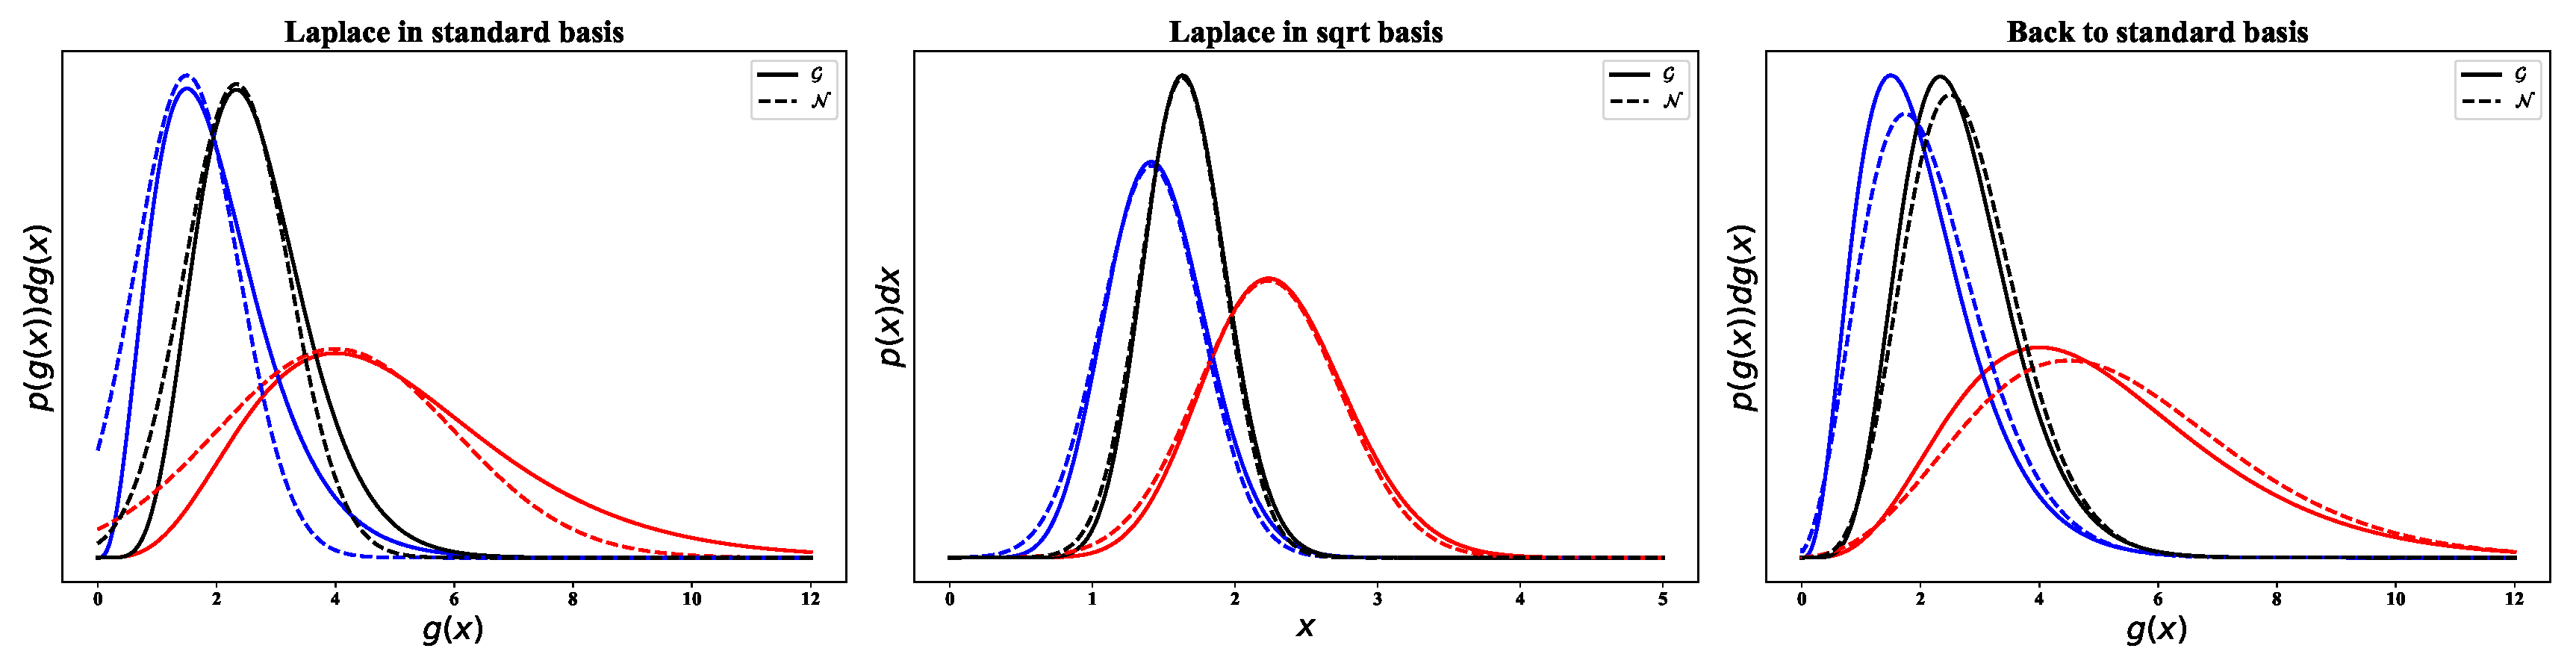
\includegraphics[width=\textwidth]{figures/gamma_bridge_sqrt.pdf}
	\caption{gamma comparison sqrt}
	\label{fig:gamma_comparison_square}
\end{figure}

\subsection{Log-Transform of the Gamma Distribution}

\subsubsection{Log-Transformation}

We transform the Gamma Distribution with the Log-Transformation, i.e. $Y = \log(X), g(x) = \log(x), g^{-1}(x) = \exp(x)$. The transformed pdf is

\begin{align}
f_Y(y, \alpha, \lambda) &= \frac{\lambda^\alpha}{\Gamma(\alpha)} \cdot y^{(\alpha - 1)} \cdot e^{(-\lambda y)} \cdot y \\ 
&=\frac{\lambda^\alpha}{\Gamma(\alpha)} \cdot y^{\alpha} \cdot e^{(-\lambda y)}
\end{align}

which can be rewritten as

\begin{equation}
f_Y(y, \alpha, \lambda) = \exp \left[\alpha \log(y) - \lambda \exp(y) \alpha \log(\lambda) - \log(\Gamma(\alpha))\right]	
\label{eq:exp_gamma_trans}
\end{equation}

with $T = (\log(y), y), \eta = (\alpha, -\lambda)$ and $A(\alpha, \lambda) = \log(\Gamma(\alpha)) - \alpha  \log(\lambda)$. 

If we insert $y = \exp(x)$ we get

\begin{align}
	f_Y(x, \alpha, \lambda) &= \cdot \exp(x)^{\alpha} \cdot e^{(-\lambda \exp(x))} \cdot \frac{1}{C}\\
	&= \exp\left[\alpha x - \lambda \exp(x) - C\right]
\end{align}

where $C$ is the integral but has no nice closed form solution.


\subsubsection{Laplace Approximation of the log-transformed Gamma Distribution}

To get the LPA of the Gamma distribution in the transformed basis we need to calculate its mode and the second derivative of the log-pdf. To get the mode we take the first derivative and set it to zero. 

\begin{align}
\text{log-pdf: } &\log\left(1/C \cdot \exp(x)^{\alpha} \cdot \exp(-\lambda \exp(x)) \right) \\
&= -C + \alpha x - \lambda \exp(x)\\
\text{1st derivative: }&  \alpha - \lambda \exp(x)\\
\text{mode: }& \alpha - \lambda \exp(x) = 0 \Leftrightarrow x = \log\left(\frac{\alpha}{\lambda}\right)\\
\text{2nd derivative: }&  -\lambda \exp(x)\\
\text{insert mode: }& -\lambda \exp(\log\left(\frac{\alpha}{\lambda}\right)) = -\alpha \\
\text{invert and times -1: }&\sigma^2 = 1/\alpha 
\end{align}

Therefore the LPA now is $N(\log\left(\frac{\alpha}{\lambda}\right), \alpha)$.

\subsubsection{The bridge for the log-transformation}

We already know how to get $\mu$ and $\sigma$ from $\lambda$ and $\alpha$. To invert we calculate $\mu = \log(\alpha/\lambda) \Leftrightarrow \lambda= \alpha/\exp(\mu)$ and insert $\alpha=\sigma^2$. In summary we have

\begin{align}
\mu &= \log(\alpha/\lambda) \\
\sigma^2 &= \alpha \\
\lambda &= \alpha/\exp(\mu) \\
\alpha &= 1/\sigma^2
\end{align}

\begin{figure}[!htb]
	\centering
	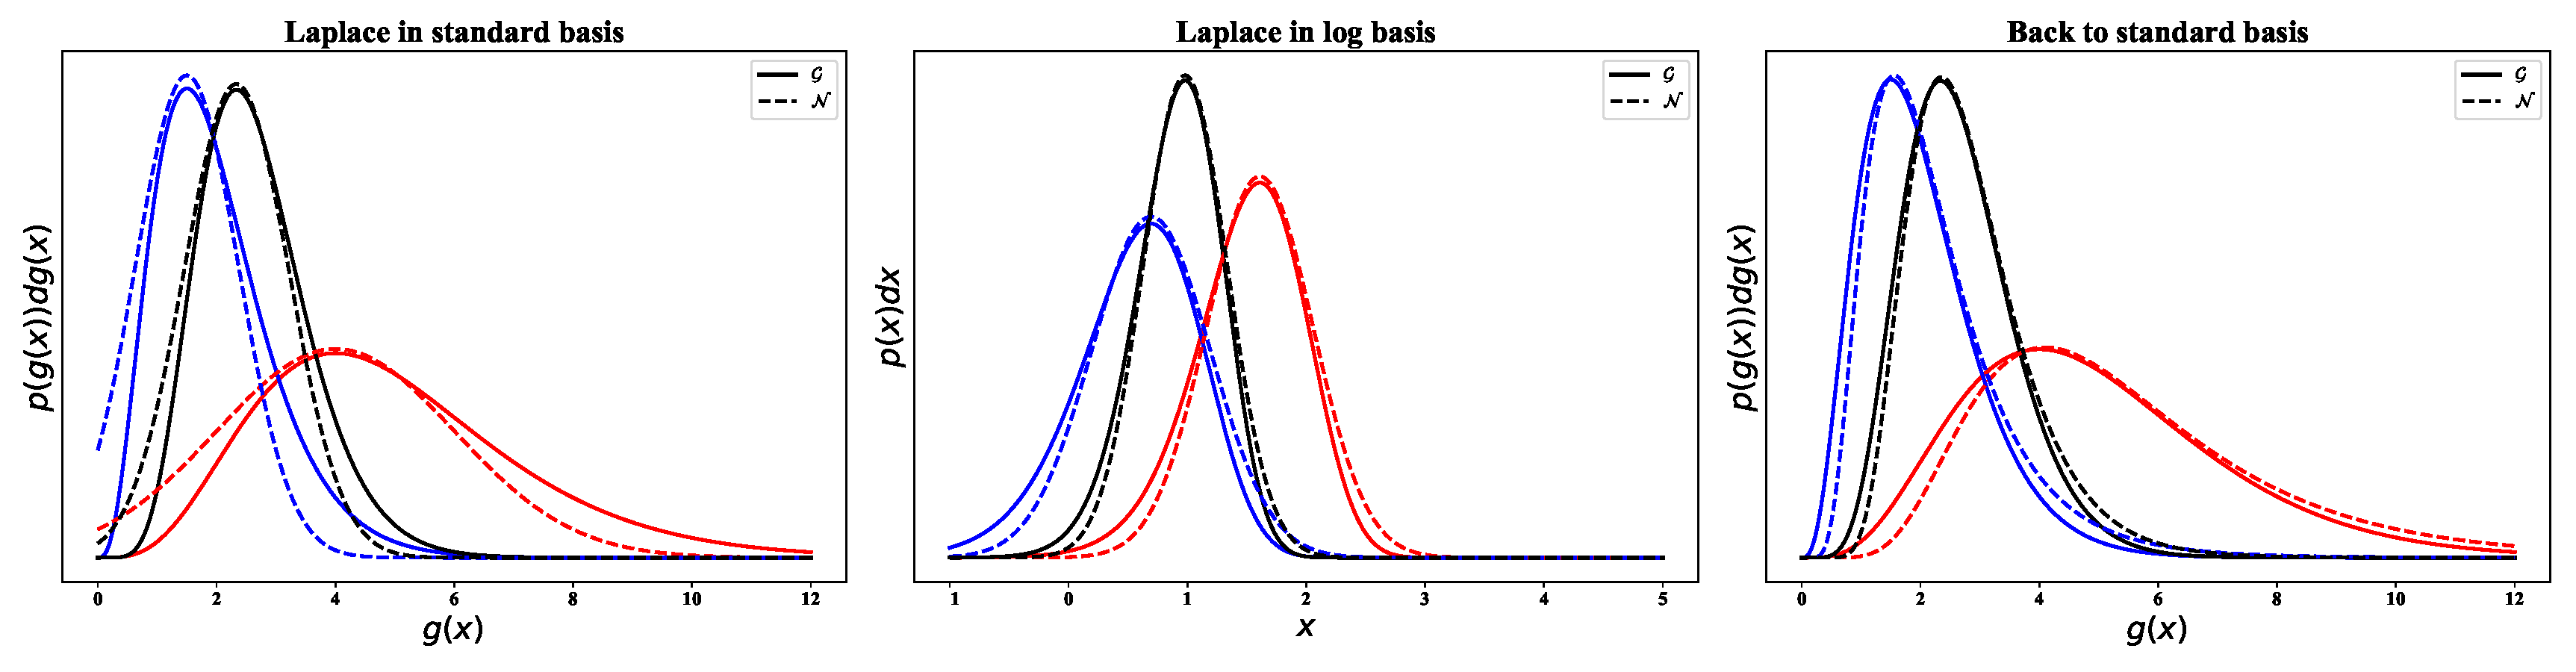
\includegraphics[width=\textwidth]{figures/gamma_bridge_log.pdf}
	\caption{gamma comparison log}
	\label{fig:gamma_comparison}
\end{figure} 


\end{document}